\chapter{Resultados}

En este capitulo se presentan los distintos resultados de este trabajo de memoria, se presentan en un orden lógico, partiendo controladores de bajo nivel, que se ejecutan el microcontrolador; y luego, el software de control que se ejecuta en el computador.

\section{Control de articulaciones}

\subsection{Control de corriente}

El lazo de corriente corresponde al \textit{loop} de control más anidado en la estructura de control distribuido propuesta, por esta razón es la que mayor ancho de banda debe presentar (más rápido). Las pruebas de control de corriente se realizaron con el rotor bloqueado, los resultados presentatos corresponden a los obtenidos en la articulación \textit{Base}.

La Figura \ref{cap5_step_corriente} muestra la respuesta del controlador de corriente ante una entrada de tipo escalón de \SI{3}{\ampere}.

\begin{figure}[h]
  \centering
  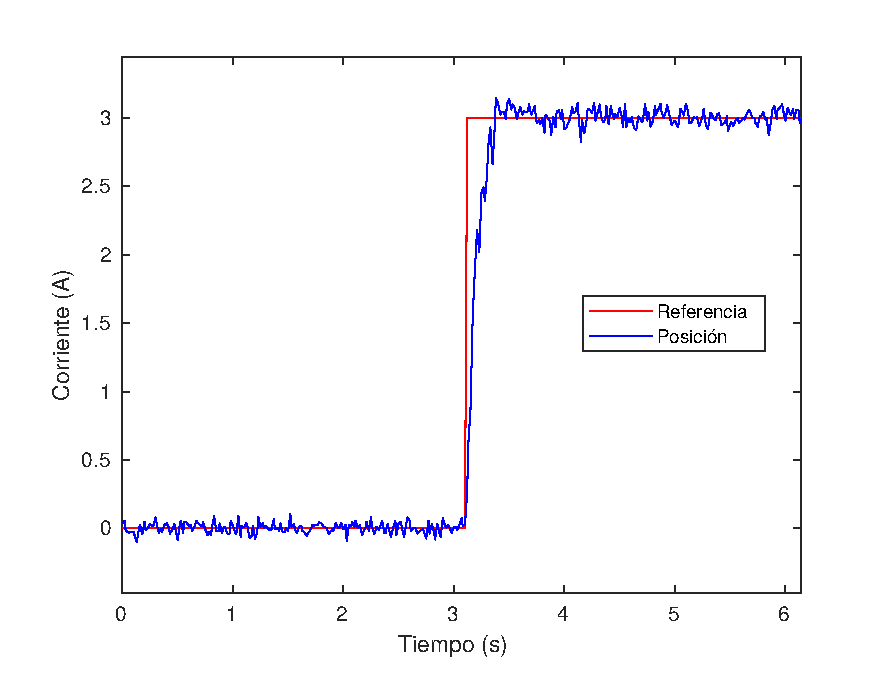
\includegraphics[width=0.5\textwidth]{img/cap5/step_corriente.pdf}
  \caption{Respuesta del controlador de corriente a un escalón.}
  \label{cap5_step_corriente}
\end{figure}

El rángo de actuación del cotrolador se há limitado a \SI{6}{\ampere}, pues corresponde a la corriente de rotor bloqueado (\textit{stall current}). La Figura \ref{cap5_corriente_cambio_referencia_alto} muestra el seguimiento de corriente a lo largo del rango de actuación durante pruebas de rotor bloqueado.

\begin{figure}[h]
  \centering
  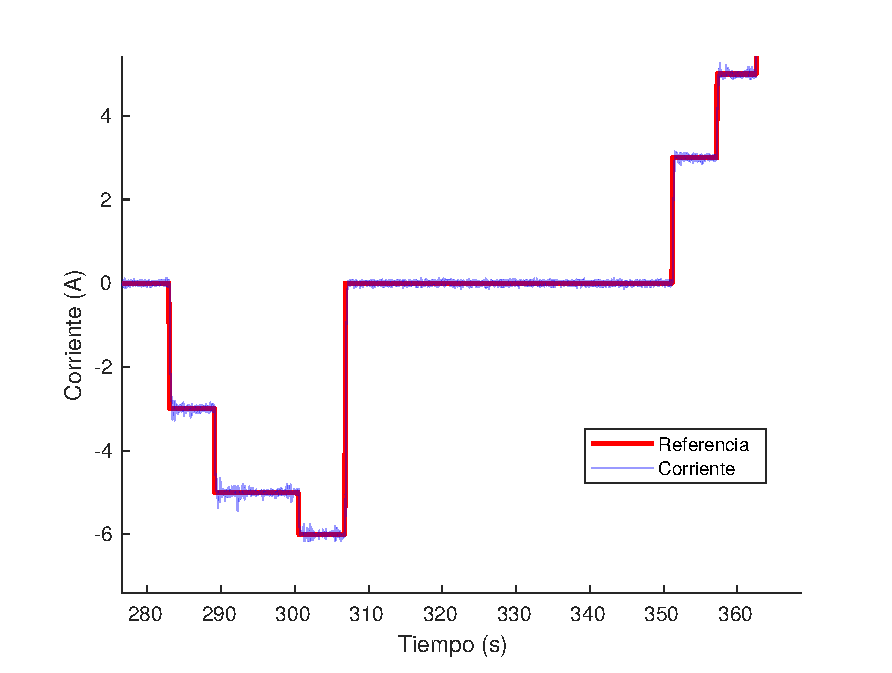
\includegraphics[width=0.5\textwidth]{img/cap5/corriente_cambio_referencia_alto.pdf}
  \caption{Respuesta del controlador de corriente ante cambios de tipo escalón en el rango completo de actuación.}
  \label{cap5_corriente_cambio_referencia_alto}
\end{figure}

Por otro lado

Seguimiento de referencia de baja amplitud
aumento del ruido por resolución del sensor
seguimiento OK

\begin{figure}[h]
  \centering
  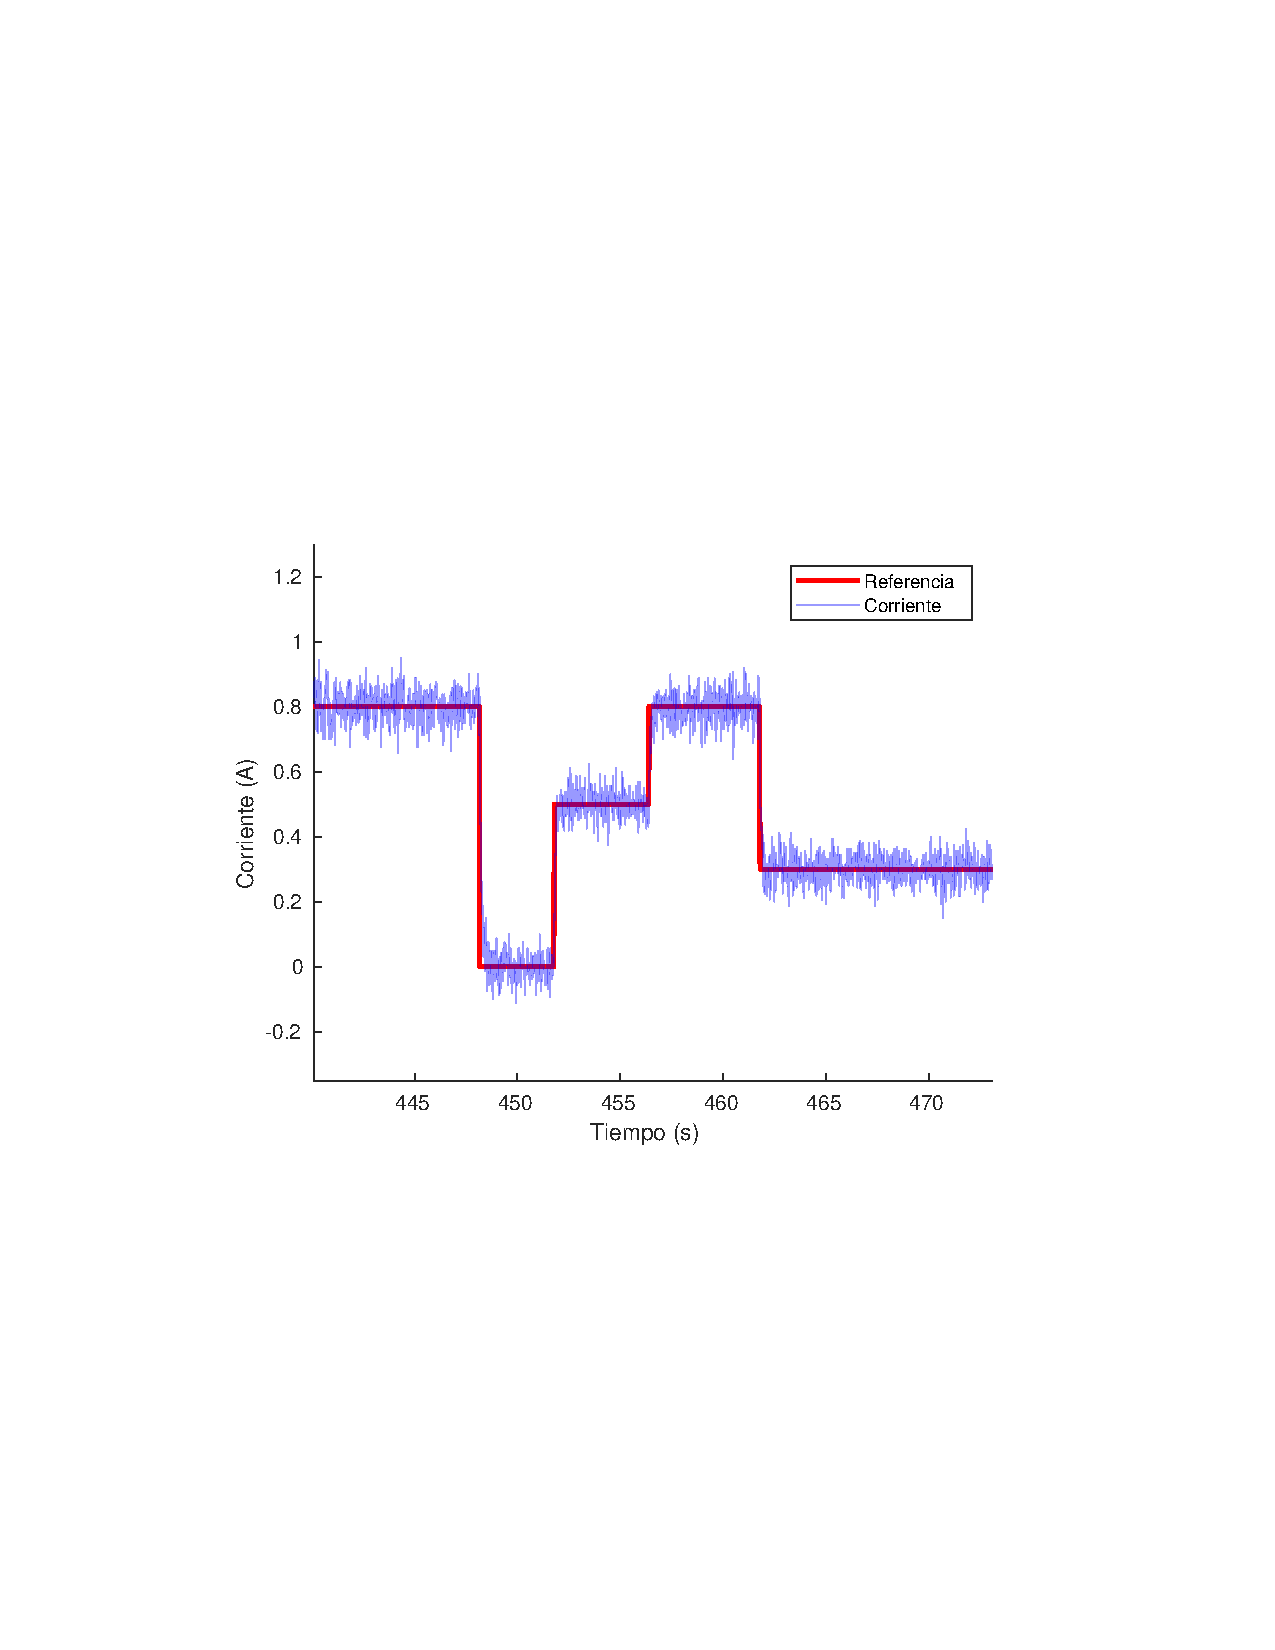
\includegraphics[width=0.5\textwidth]{img/cap5/corriente_cambio_referencia_bajo.pdf}
  \caption{Respuesta del controlador de corriente a un escalón.}
  \label{cap5_corriente_cambio_referencia_bajo}
\end{figure}




Cambio dinamico
pruebas realizadas con rotor bloqueado
movimiento induce que no se pueda alcanzar la corriente por falta de carga, antiwindup debe actuar

\begin{figure}[h]
  \centering
  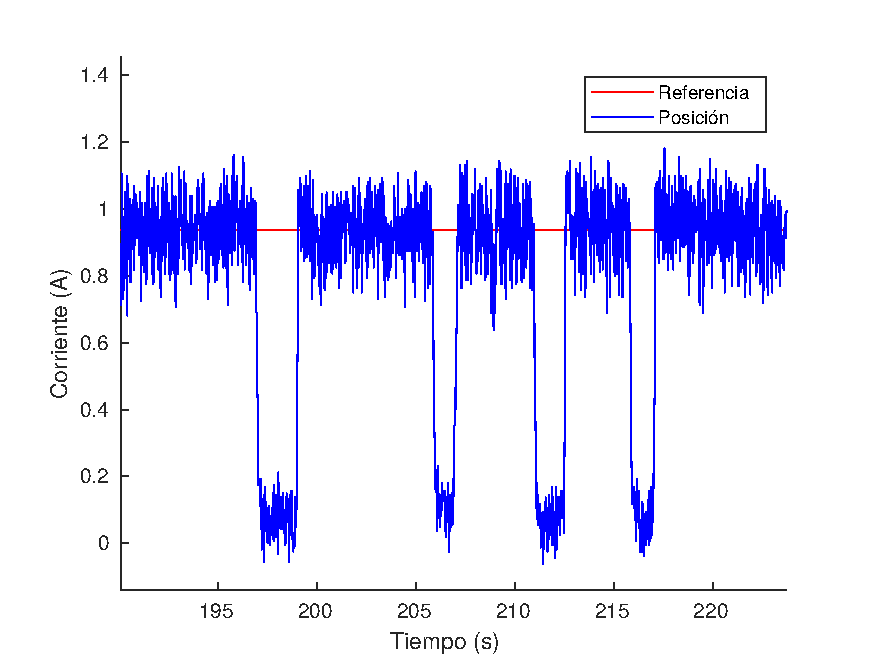
\includegraphics[width=0.5\textwidth]{img/cap5/cambio_dinamico_corriente.pdf}
  \caption{Respuesta del controlador de corriente a un escalón.}
  \label{cap5_cambio_dinamico_corriente}
\end{figure}


\subsection{Control de velocidad}

\subsection{Control de posición}

\begin{figure}[H]
  \centering
  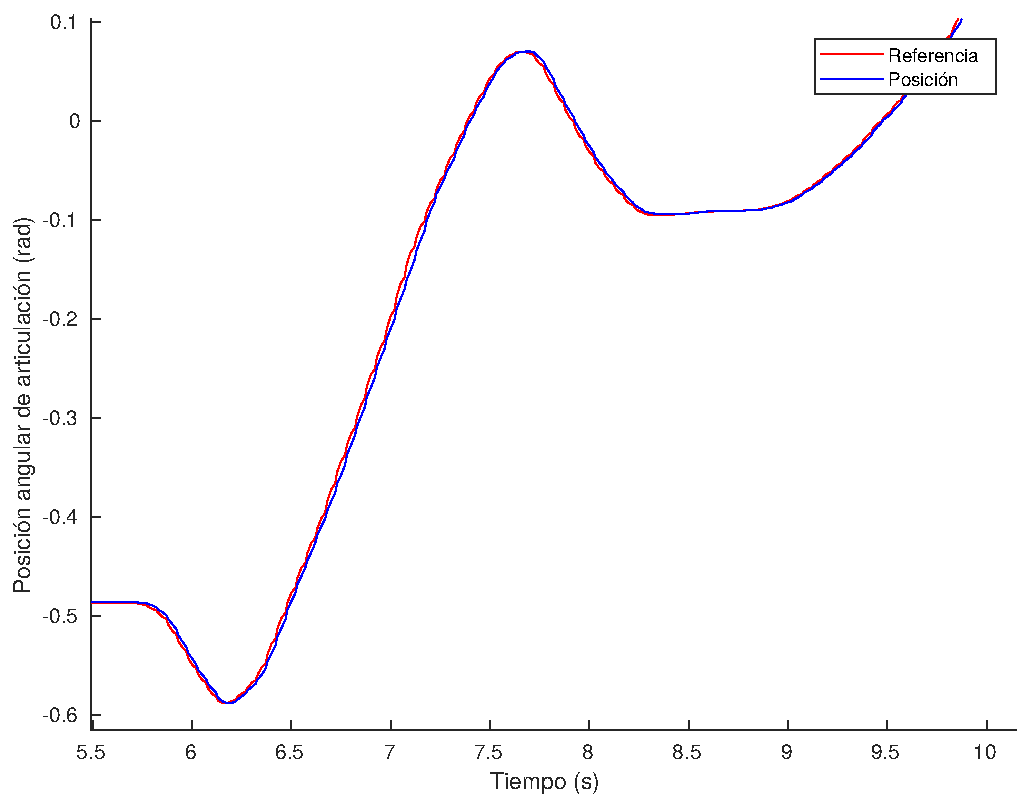
\includegraphics[width=0.5\textwidth]{img/cap5/ref_basica}
  \caption{Respuesta del controlador de corriente a un escalón.}
  \label{cap5_ref_basica}
\end{figure}



\begin{figure}[H]
  \centering
  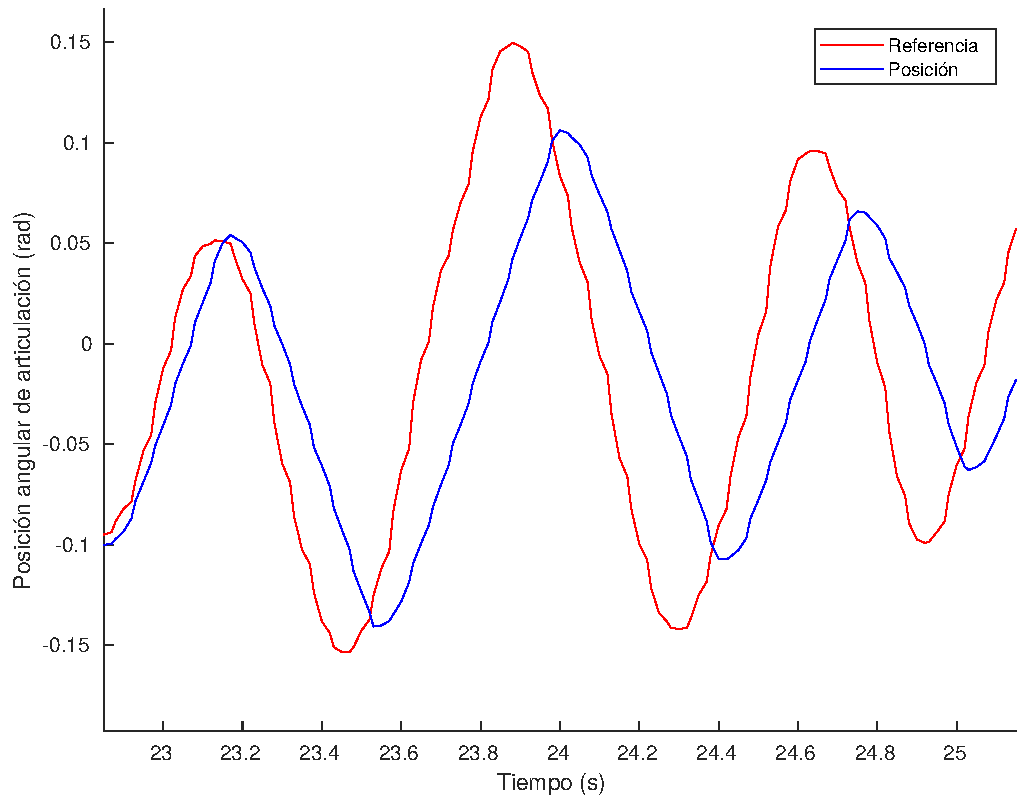
\includegraphics[width=0.5\textwidth]{img/cap5/ref_retardo_vel}
  \caption{Respuesta del controlador de corriente a un escalón.}
  \label{cap5_ref_retardo_vel}
\end{figure}

\begin{figure}[H]
  \centering
  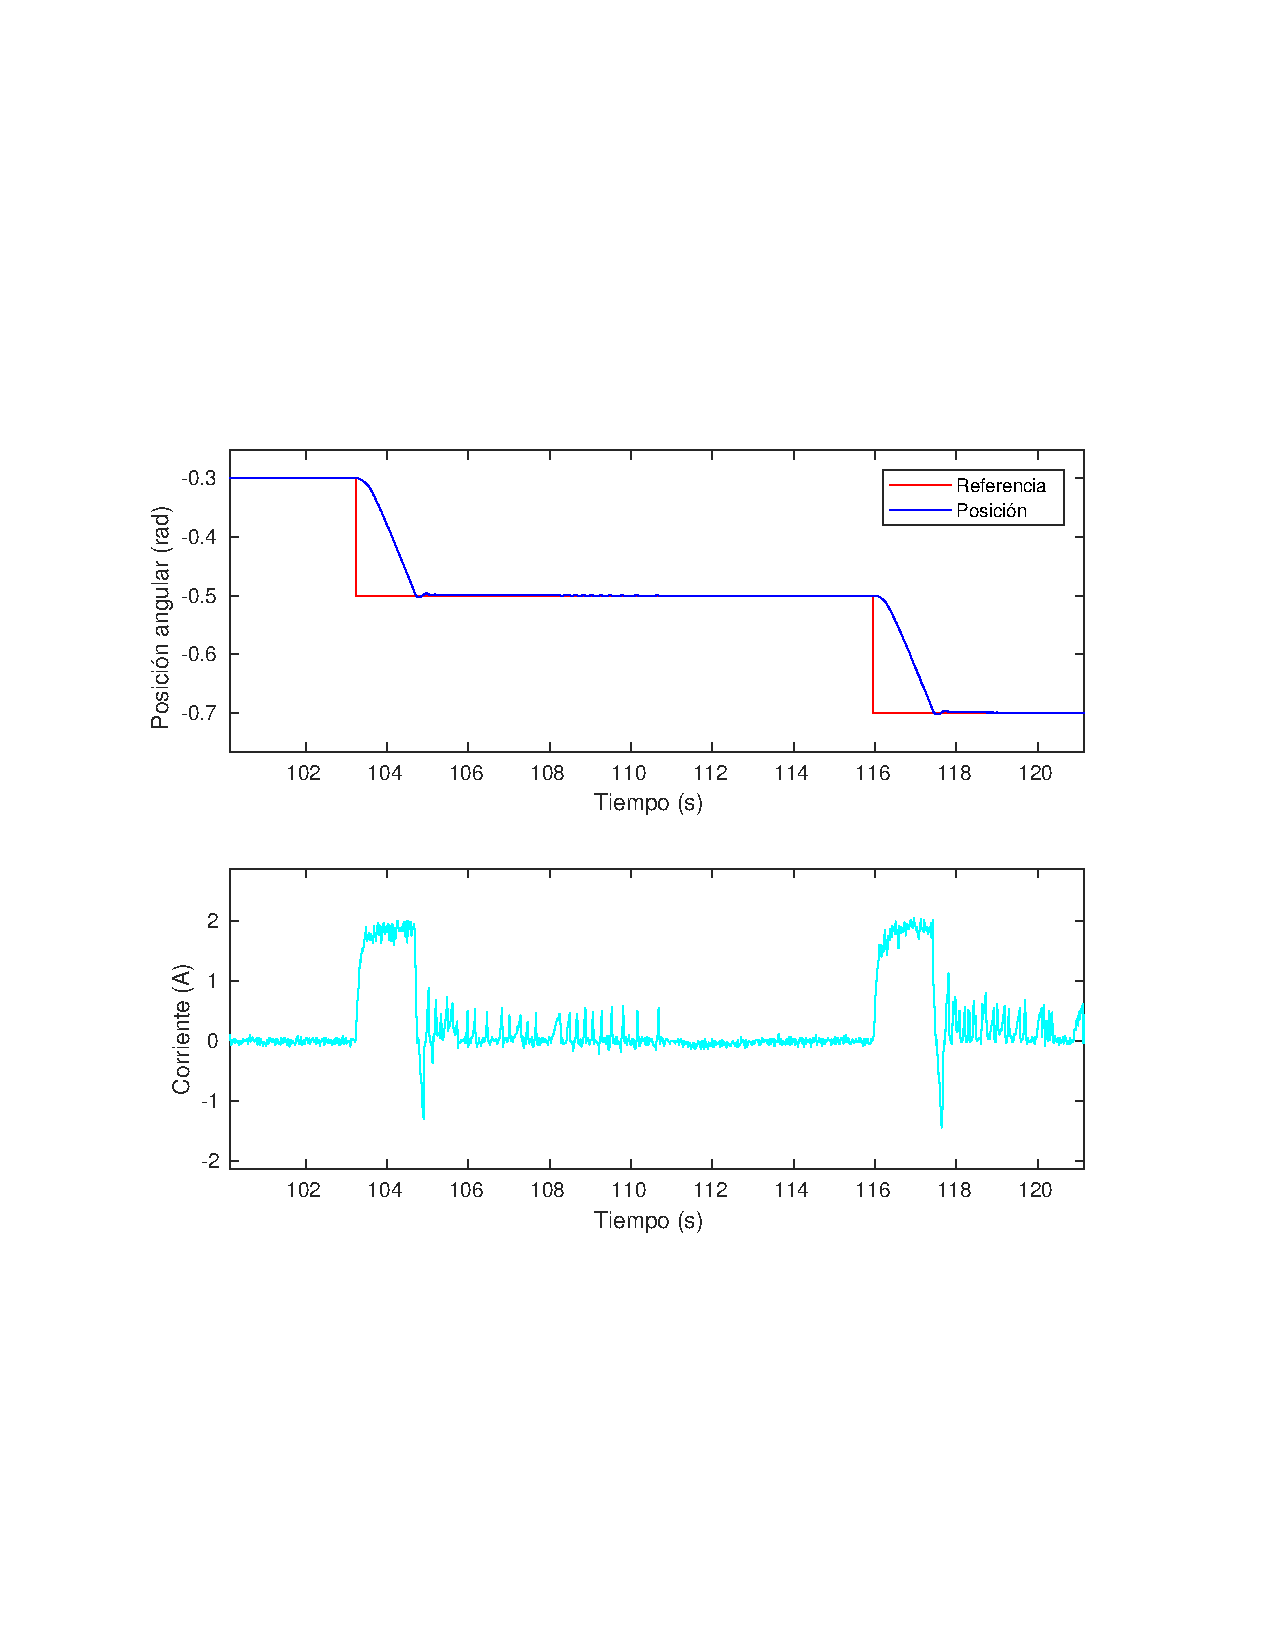
\includegraphics[width=0.8\textwidth]{img/cap5/ref_corriente_limitada}
  \caption{Respuesta del controlador de corriente a un escalón.}
  \label{cap5_ref_corriente_limitada}
\end{figure}

\section{Control mediante Phantom Omni}

\subsection{Mapeo de articulaciones}

\begin{figure}[H]
  \centering
  \begin{subfigure}[b]{0.35\textwidth}
    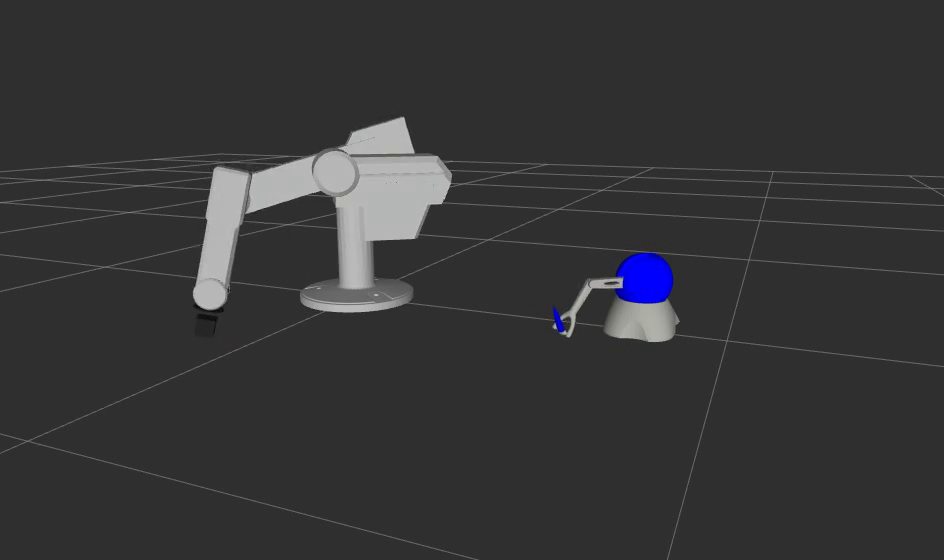
\includegraphics[width=0.9\textwidth]{img/cap5/mapping_01}
    \caption{}
  \end{subfigure}%
  \quad
  \begin{subfigure}[b]{0.35\textwidth}
    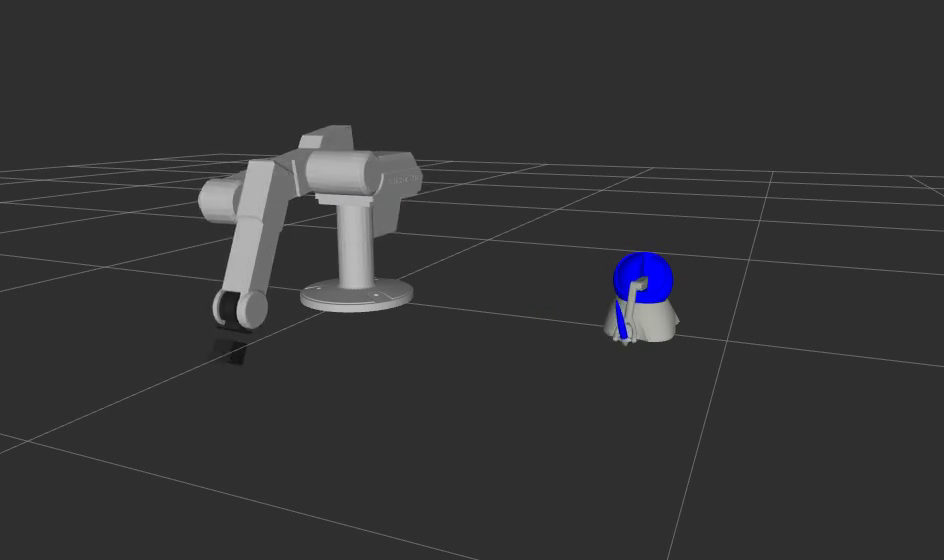
\includegraphics[width=0.9\textwidth]{img/cap5/mapping_02}
    \caption{}
  \end{subfigure}
  \vskip\baselineskip
  \begin{subfigure}[b]{0.35\textwidth}
    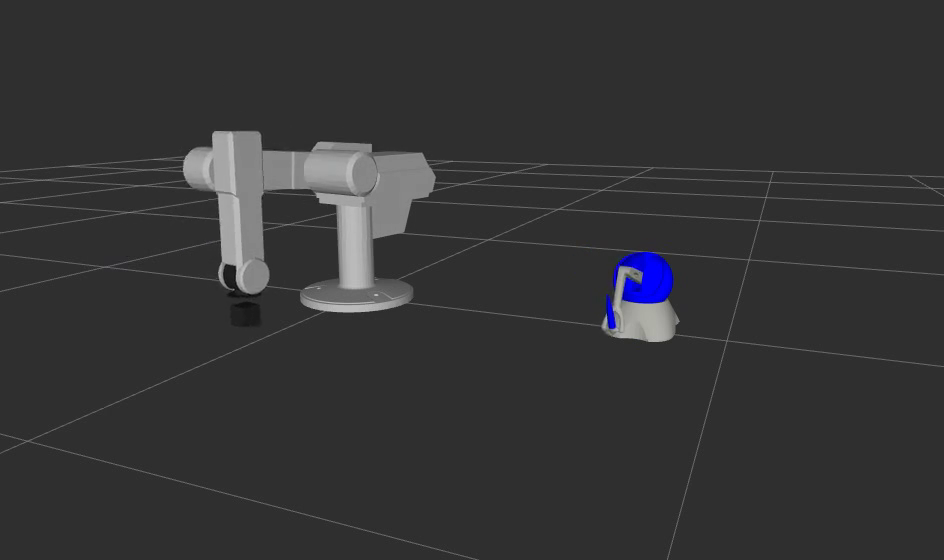
\includegraphics[width=0.9\textwidth]{img/cap5/mapping_03}
    \caption{}
  \end{subfigure}%
  \quad
  \begin{subfigure}[b]{0.35\textwidth}
    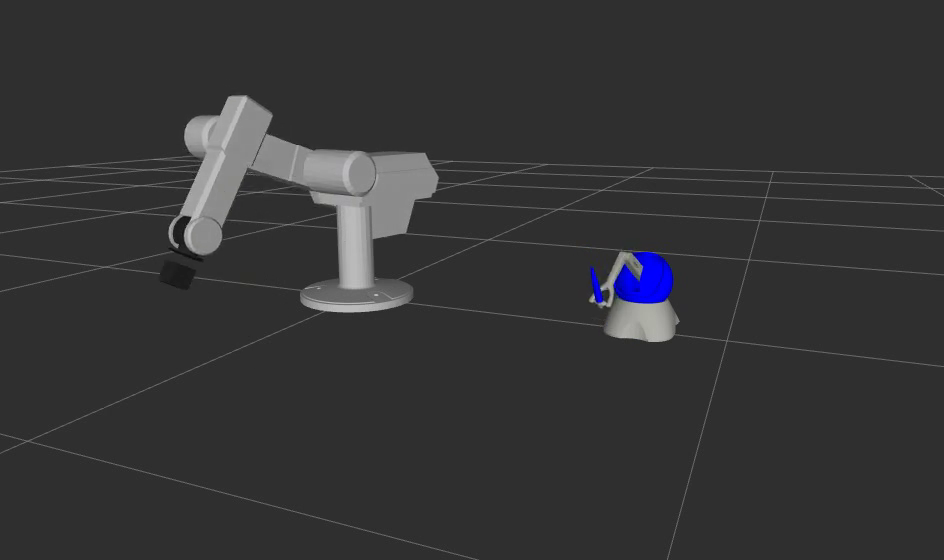
\includegraphics[width=0.9\textwidth]{img/cap5/mapping_04}
    \caption{}
  \end{subfigure}
  \caption{Mapeo de articulaciones entre el Phantom Omni y el robot Scorbot.}
  \label{cap5_joint_mapping}
\end{figure}


\subsection{Feedback haptico}

\begin{figure}[H]
  \centering
  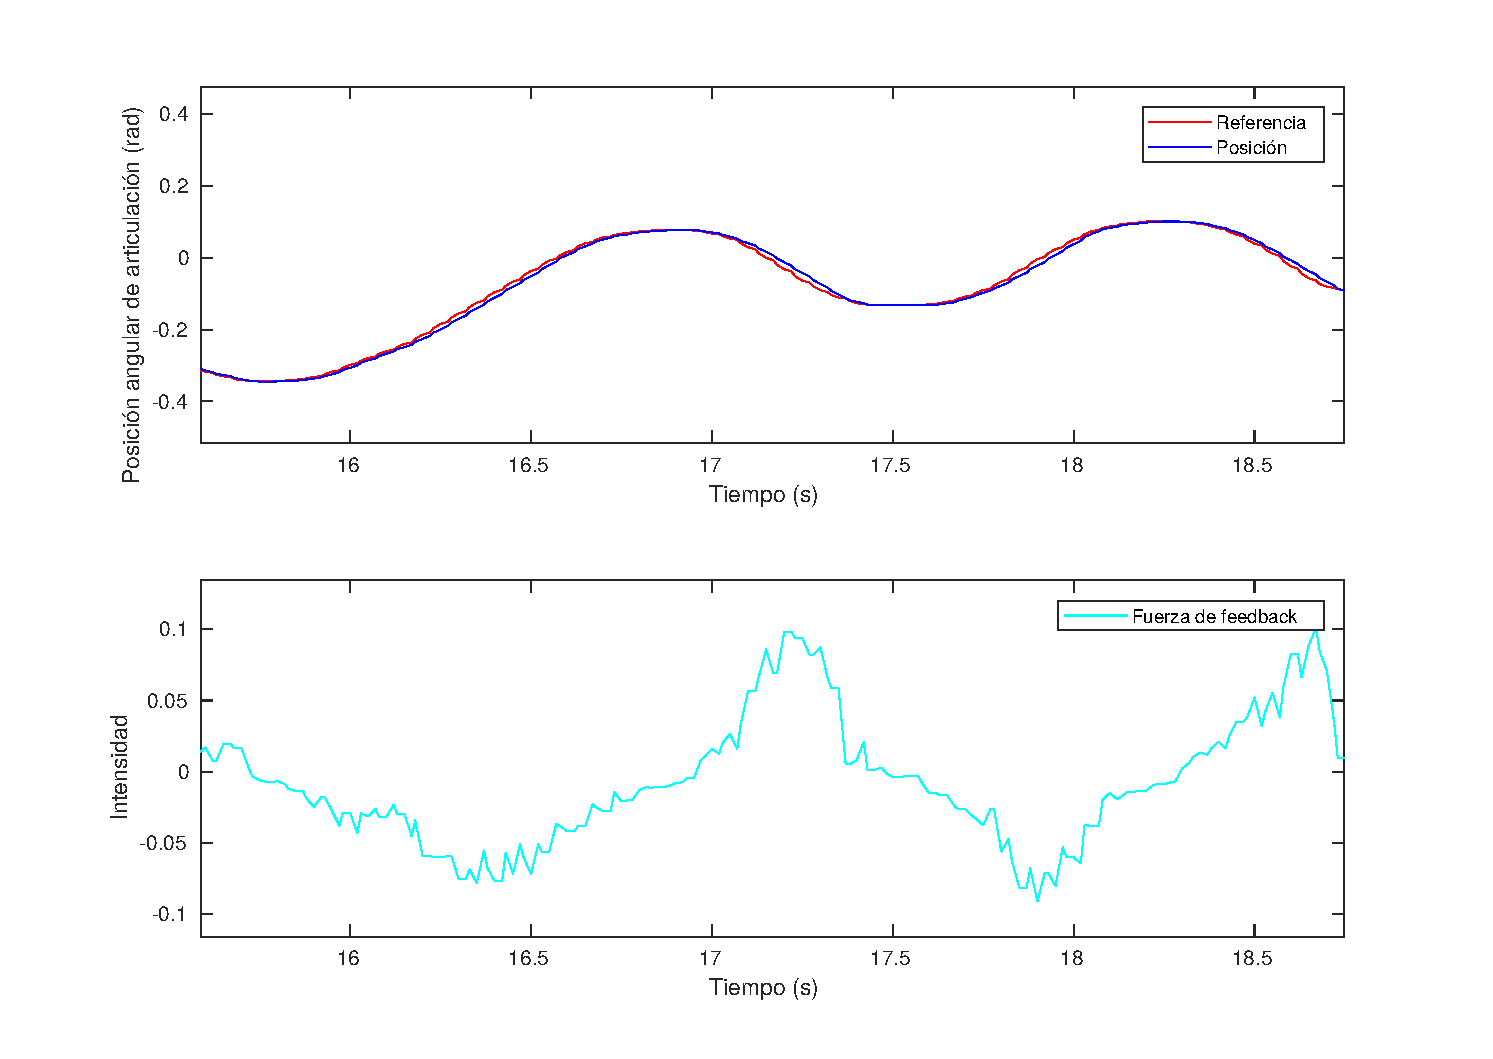
\includegraphics[width=0.5\textwidth]{img/cap5/feedback_basico}
  \caption{Algoritmo de fuerza.}
  \label{cap5_feedback_basico}
\end{figure}


\begin{figure}[H]
  \centering
  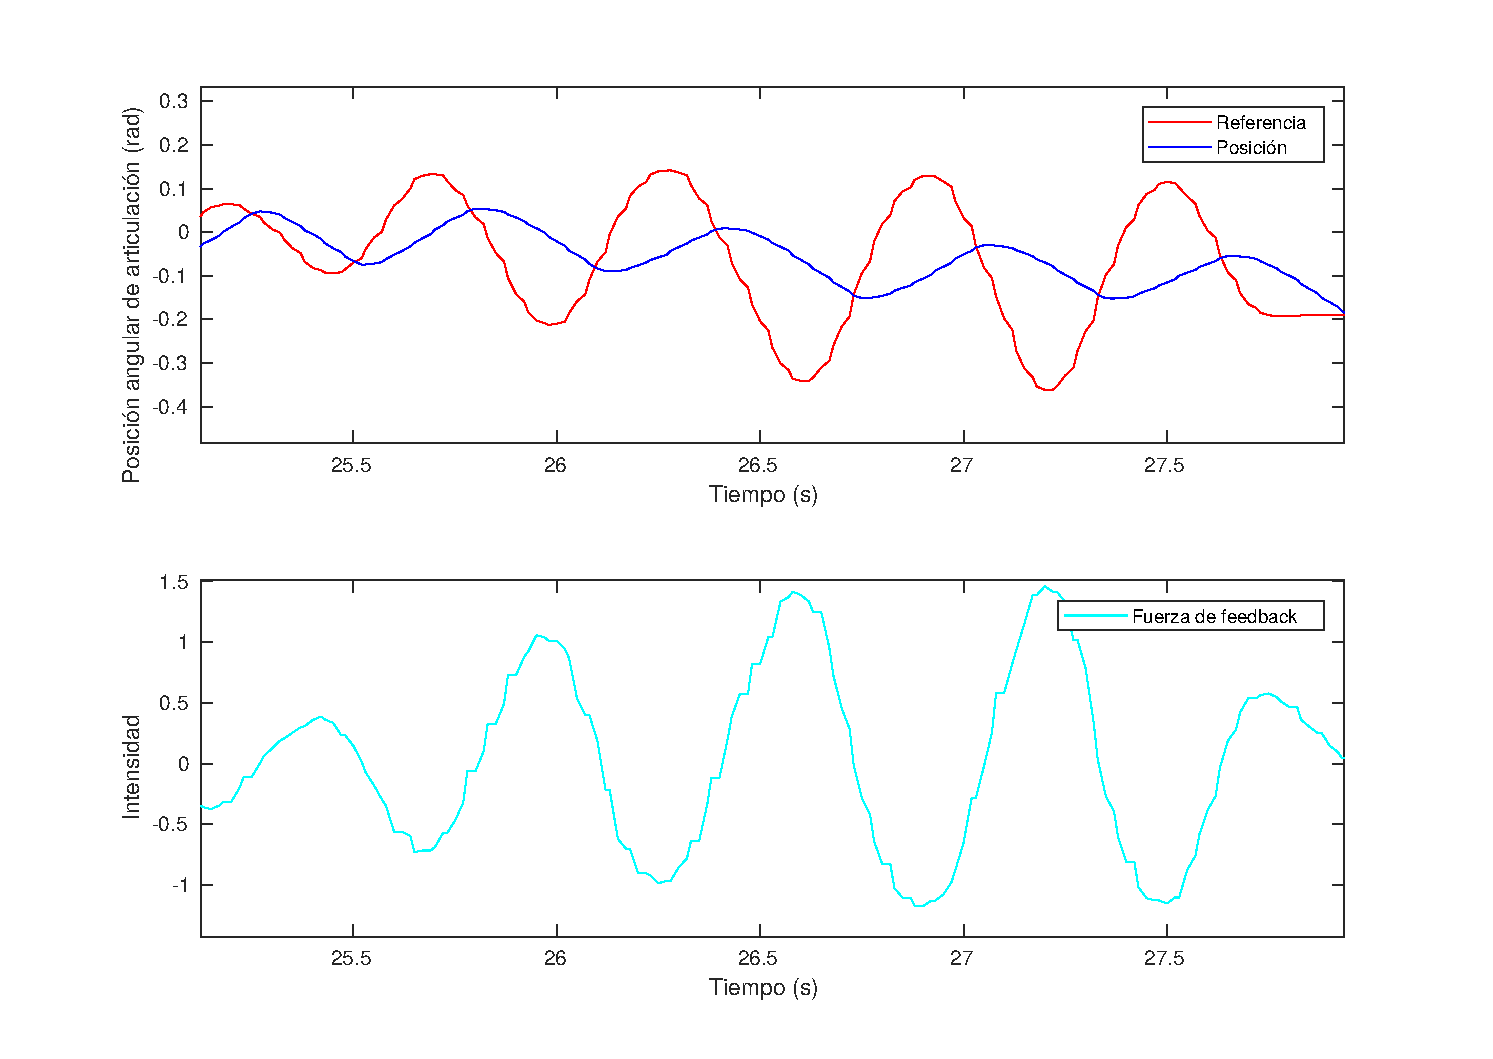
\includegraphics[width=0.5\textwidth]{img/cap5/feedback_velocidad}
  \caption{Seguimiento de trayectoria con aplicación de fuerza.}
  \label{cap4_force_tracking}
\end{figure}




